\documentclass{Academic}
\usepackage{csquotes}
\usepackage{algorithm}
\usepackage{algpseudocode}

\addbibresource{references.bib}

\begin{document}
%Easy customisation of title page
%TC:ignore
    \myabstract{%\small
%\noindent\textbf{Abstract}
%%Abstract below
%
%The hypothesis/question and its context, scope and significance are briefly and precisely defined. The main conclusions are brief, precise and clear, noting methods used and key results. The language is clear, precise and easy to understand with no irrelevant information.}
    \renewcommand{\myTitle}{Hybrid Recommender Models in E-Learning: A Comprehensive Review of HybridBERT4Rec}
    \renewcommand{\MyAuthor}{Leon Knorr}
    \renewcommand{\MyDepartment}{Mannheim Master of Datascience}
    \renewcommand{\ID}{1902854}
    \renewcommand{\Keywords}{Education, AI, E-Learning}
    \maketitle
%\vspace{-1.9em}\noindent\rule{\textwidth}{1pt} %add this line if not using abstract
    %\onehalfspacing
%TC:endignore

    \section{Introduction}
    In the dynamic landscape of today's knowledge-driven society and global economics, the concept of life-long learning has evolved into a cornerstone for personal and professional development. It ensures the competitiveness of individuals in a globalized market, while also aiding in overcoming social challenges, such as demographic change, social cohesion or public health through continuous education. Because of its key-role in overcoming today's challenges, many governments and corporations invested heavily in lifelong learning offerings and frameworks \cite{rubensonAdultLearningEducation2011}. This investment can be seen by observing the vast landscape of different learning platforms, which have emerged over the last couple of years, ranging from publicly funded E-Learning solutions such as Moodle\cite{StartseiteMoodleOrg} or ILIAS\cite{Ilias}, to private corporate platforms such as Linked-In Learning\cite{LinkedInLearningMit}. As individuals embark on continuous learning journeys on such platforms, the demand for tailored educational experiences has surged. These experiences not only include the recommendation of new content, but also content which aims to aid the user with current learning objectives. Recommender algorithms play a pivotal role in shaping these learning odysseys by providing personalized content recommendations \cite{jeevamolOntologybasedHybridElearning2021}. \\
    In this work, the hybrid content recommendation system HybridBERT4Rec, which uses a transformer based approach to collaborative and content-based filtering techniques, is reviewed and adapted to an E-Learning use case.

    \section{Related Work}

    \section{Sequential Content Recommendation}
    Traditional content recommendation systems usually observe user interactions as a set of independent and unrelated data points. These systems then compute or form a hidden representation in order to model user interests, which can then be used to predict which items may be relevant for the given user. If an item is considered relevant, it gets recommended. This modeling technique models a user's \textit{general} preferences and interests \cite{wangSequentialRecommenderSystems2019}. But, this is insufficient modelling, as user preferences change over time \cite{wangSequentialRecommenderSystems2019}! For example, let Alice be a user whose general interests reflect romantic films, such as Titanic, Romeo \& Juliet or \enquote{me before you} and who recently got into the Marvel Universe, and started watching Movies like \enquote{Spider-Man}. In addition, Alice is now really interested in following up with that series. Alice's movie history contains a total of 10 movies, 9 romantic movies and one Spider-Man movie, with the latter being the most recently watched. A traditional content recommendation system would observe Alice's movie history and model her interests as consisting of 90\% romantic films and 10\% Marvel. As a result, the recommendation system would assign romantic films a higher relevance score than a movie that is similar to Spider-Man, leading to unsatisfying recommendations for Alice's \textit{current} interests. Sequential Content Recommendation aims to solve this problem by modelling user-interactions as a sequence.

    \begin{figure}[ht!]
        \centering
        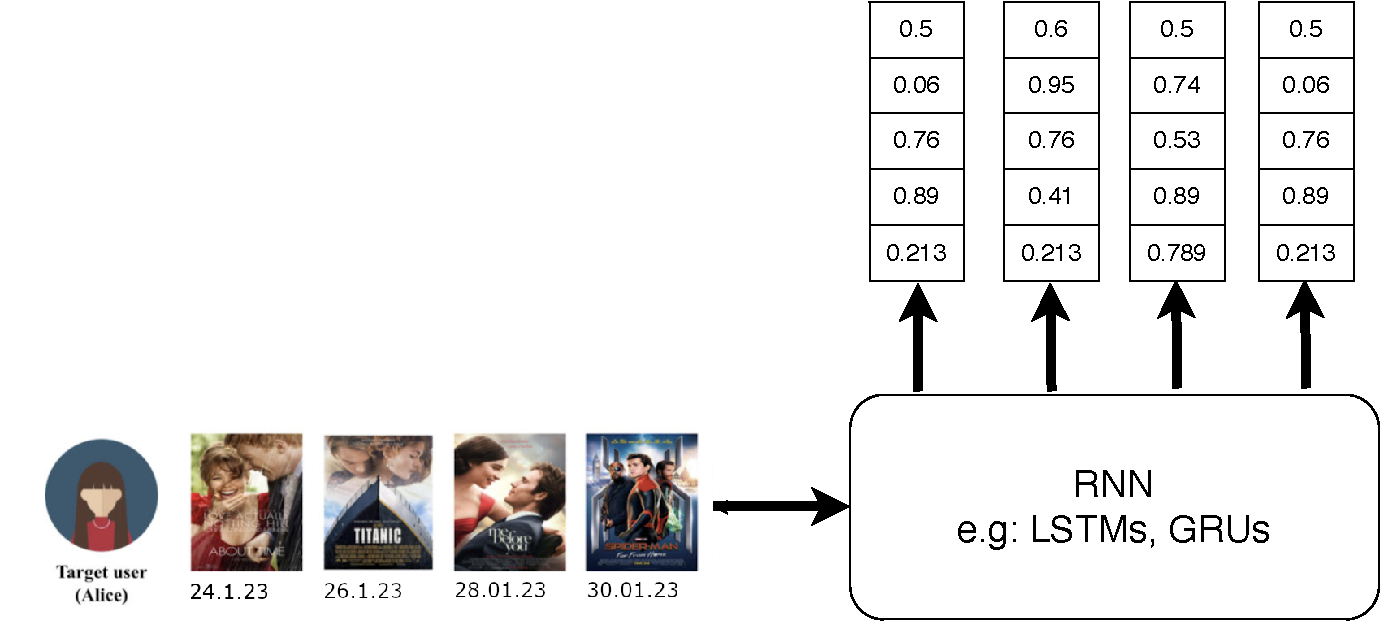
\includegraphics[width=0.6\textwidth]{images/rnn_seq.pdf}
        \caption{Sequential Content Recommendation with RNNs \cite{yuDynamicRecurrentModel2016}}
        \label{fig:seqRNN}
    \end{figure}

    \FloatBarrier

    \section{HybridBERT4Rec}
        \begin{figure}[ht!]
            \centering
            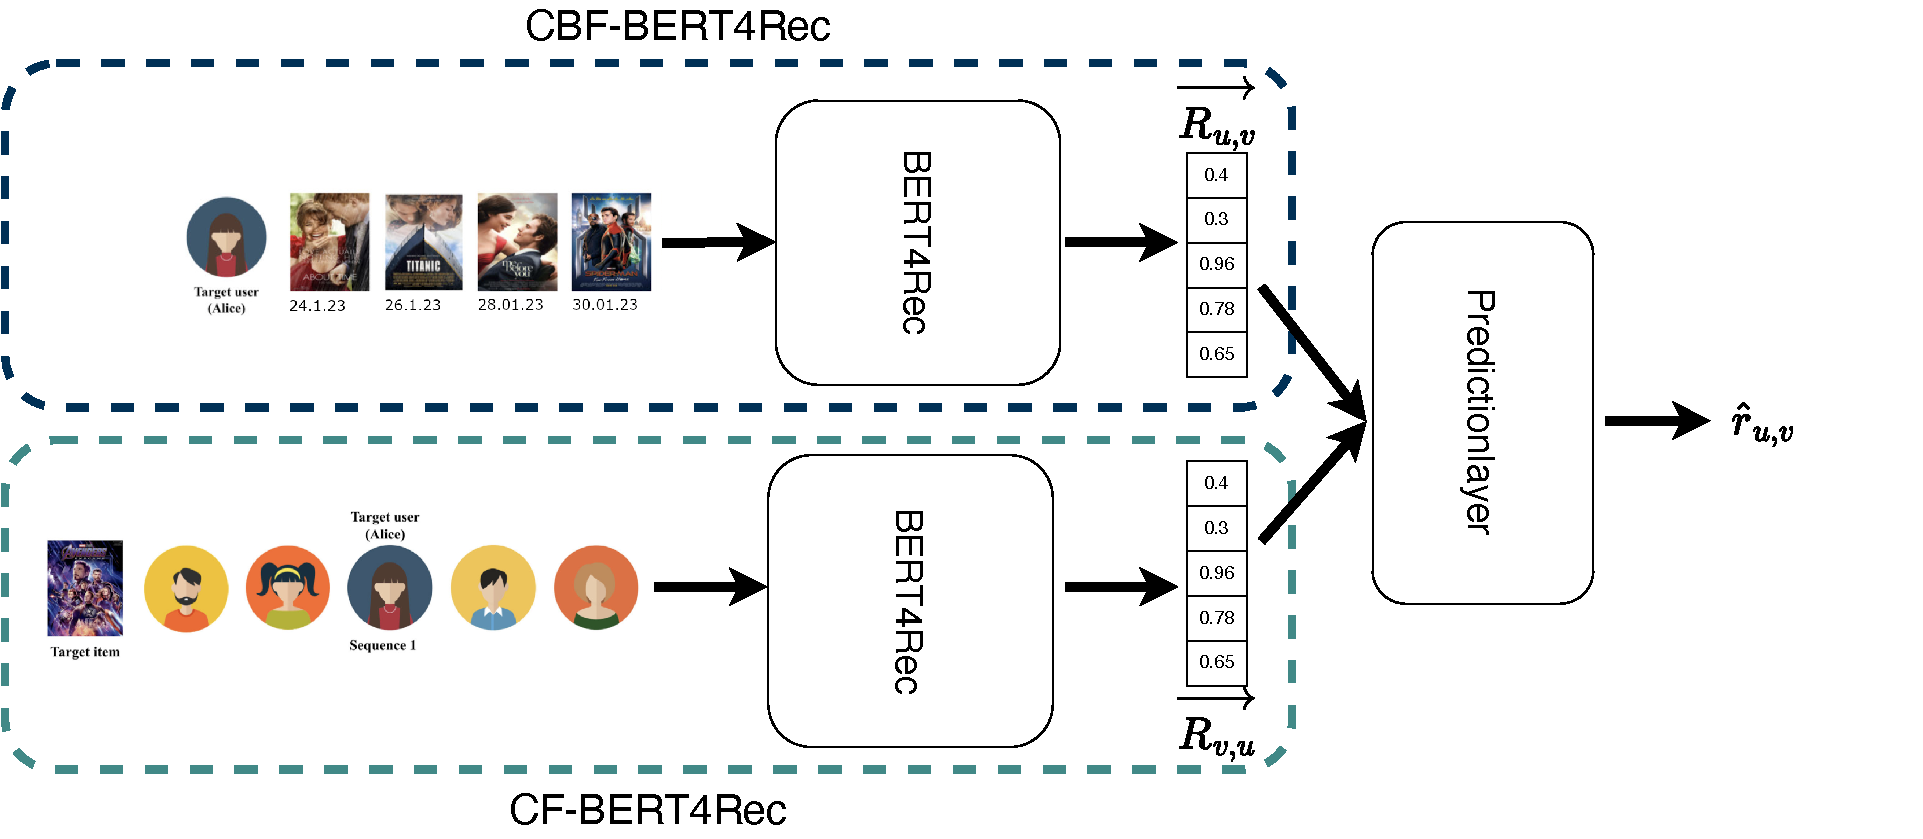
\includegraphics[width=0.6\textwidth]{images/hybridBERT4Rec_high_level.pdf}
            \caption{High level overview of HybridBERT4Recs Architecture. \cite{channarongHybridBERT4RecHybridContentBased2022}}
            \label{fig:highlevel}
        \end{figure}

        \subsection{BERT4Rec}
        \begin{figure}[ht!]
            \centering
            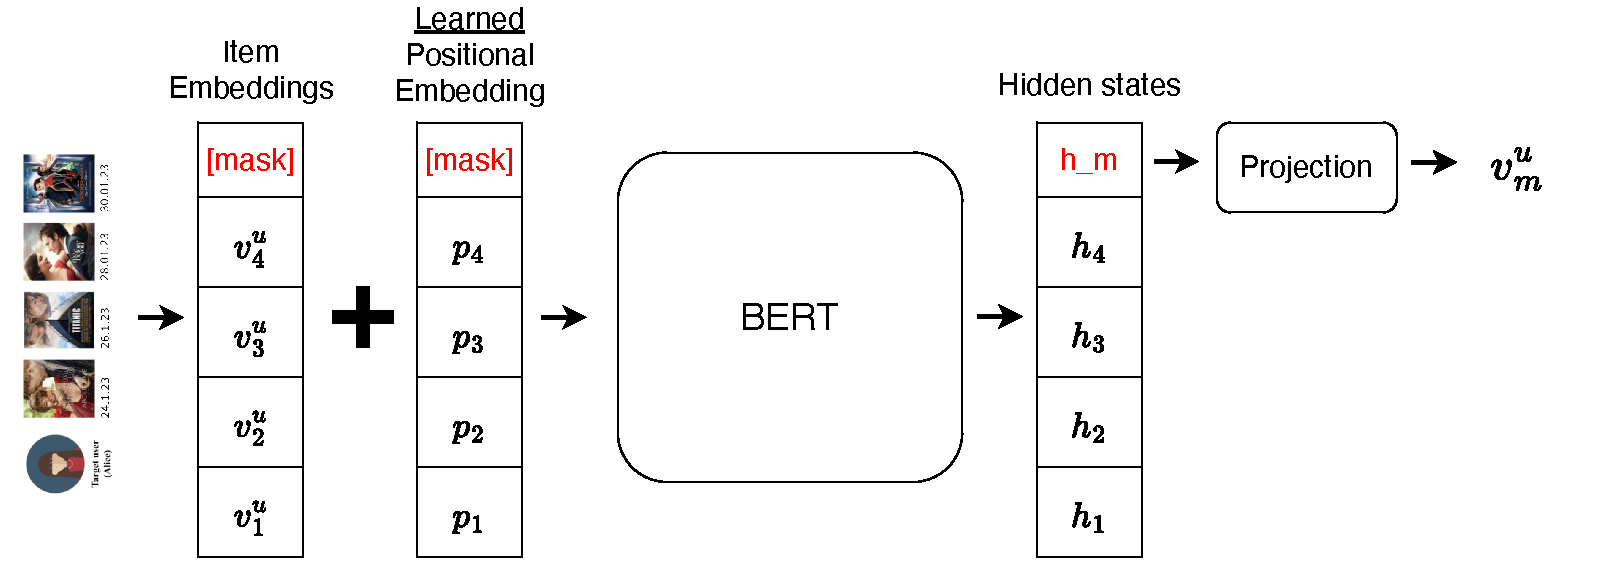
\includegraphics[width=0.6\textwidth]{images/BERT4Rec.pdf}
            \caption{BERT4Rec Architecture, taking item embeddings $v_t^u$ from user $u$'s history as input and predicts the next item $v_m^u$, u is likely to interact with \cite{sunBERT4RecSequentialRecommendation2019}.}
            \label{fig:bert4rec}
        \end{figure}

        \subsection{CF-HybridBERT4Rec}
        \begin{figure}[ht!]
            \centering
            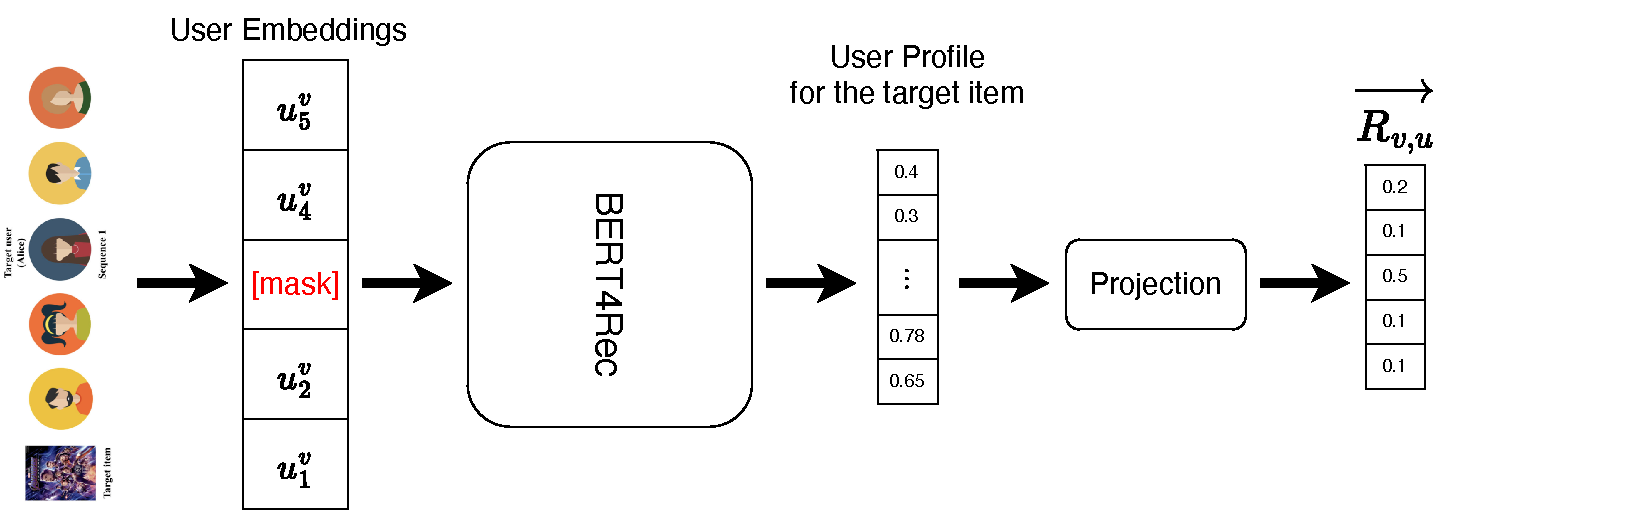
\includegraphics[width=0.6\textwidth]{images/CF-HybridBERT4Rec.pdf}
            \caption{CF-HybridBERT4Rec Architecture, taking user embeddings from all users that have rated the target item $v$ as input and predicts the \enquote{target item profile $\overrightarrow{R_{v,u}}$} \cite{channarongHybridBERT4RecHybridContentBased2022}.}
            \label{fig:cf-arch}
        \end{figure}

        \subsection{CBF-HybridBERT4Rec}
        \begin{figure}[ht!]
            \centering
            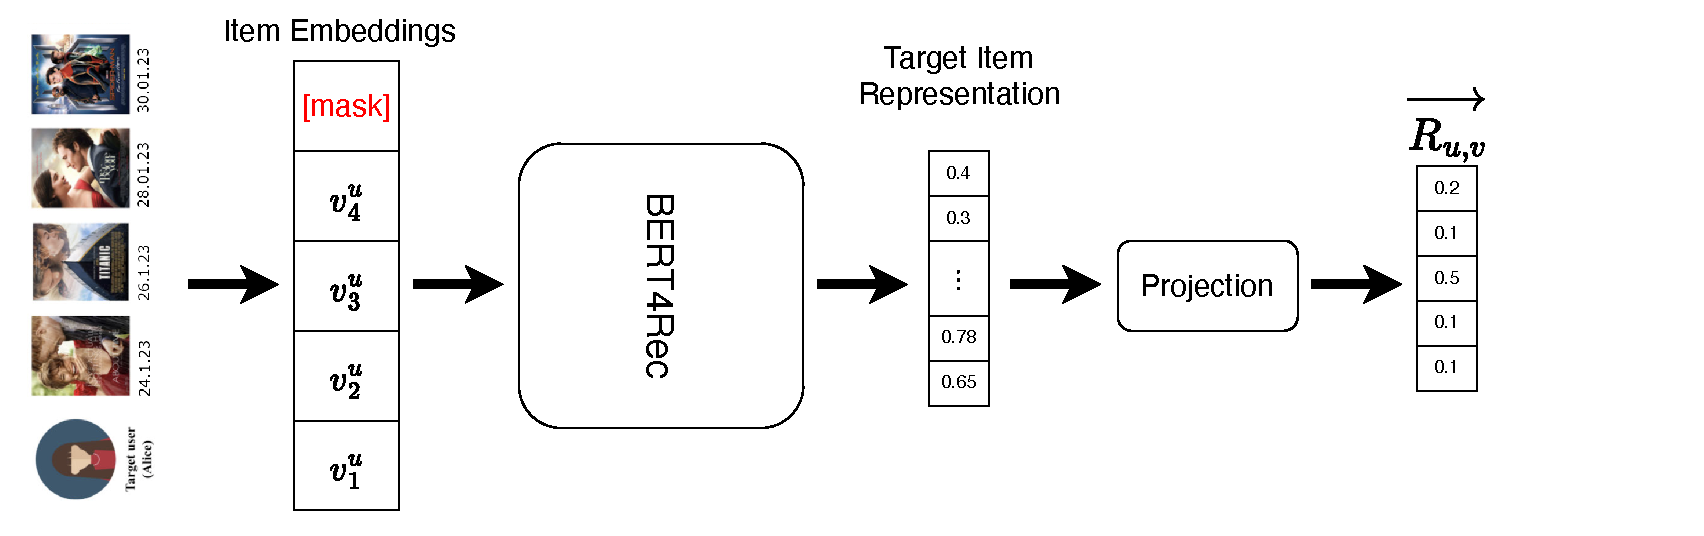
\includegraphics[width=0.6\textwidth]{images/CBF-HybridBERT4Rec.pdf}
            \caption{CBF-HybridBERT4Rec Architecture, taking item embeddings from a user $u$ history as input and predicts a \enquote{target user profile $\overrightarrow{R_{u,v}}$} \cite{channarongHybridBERT4RecHybridContentBased2022}.}
            \label{fig:cbf-arch}
        \end{figure}

        \subsection{Prediction Layer}
        \begin{figure}[ht!]
            \centering
            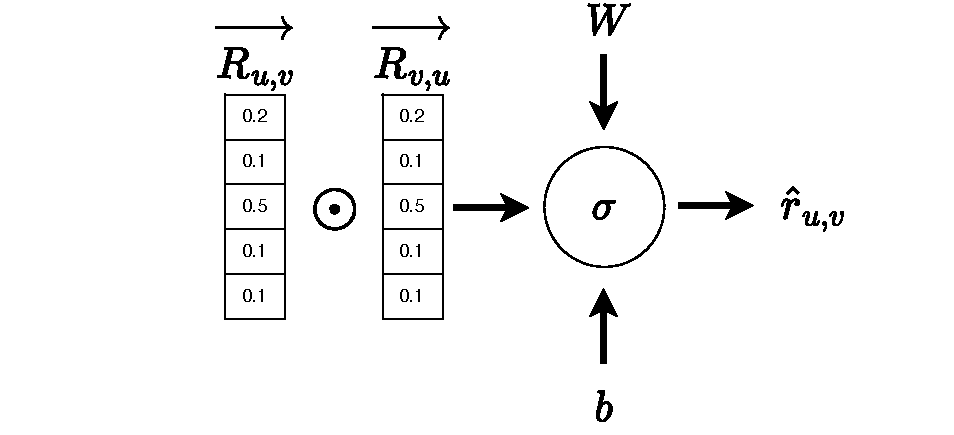
\includegraphics[width=0.5\textwidth]{images/Prediction_Layer.pdf}
            \caption{Schematic of HybridBERT4Recs Prediction layer, which uses a generalization of Matrix Factorization based on Neural Networks with Sigmoid activations to predict the rating $\hat{r}_{u,v}$ user $u$ would assign to item $v$ \cite{channarongHybridBERT4RecHybridContentBased2022}.}
            \label{fig:pred_layer}
        \end{figure}
        \begin{equation}
            \hat{r}_{u,v} = \sigma(WR(u,v) + b), \text{ with }
            R(u,v) = R_{uv} \odot R_{vu}
        \end{equation}

        \subsection{Strengths \& Weaknesses}

        \subsection{Performance \& Experiments}
        \begin{figure}[ht!]
            \centering
			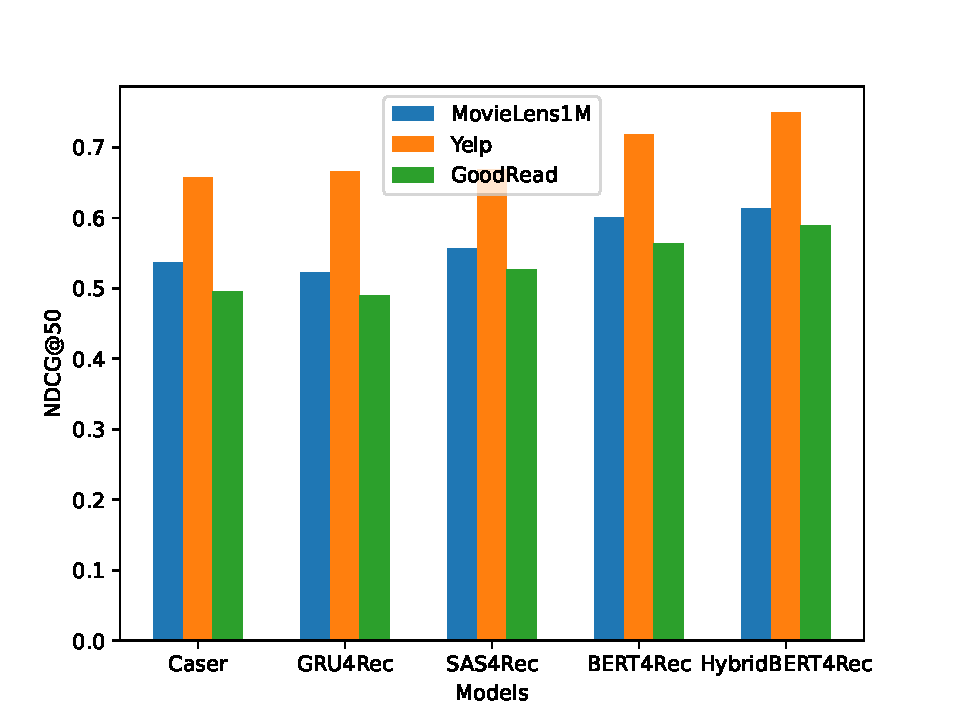
\includegraphics[width=0.6\textwidth]{images/results.pdf}
			\caption{Performance comparison of different recommender models on three datasets as published by the authors of HybridBERT4Rec \cite{channarongHybridBERT4RecHybridContentBased2022}.}
            \label{fig:perfExp}
		\end{figure}

    \section{Applying HybridBERT4Rec in an E-Learning Environment}

        \subsection{The Trivial Solution}
        \begin{figure}[ht!]
            \centering
			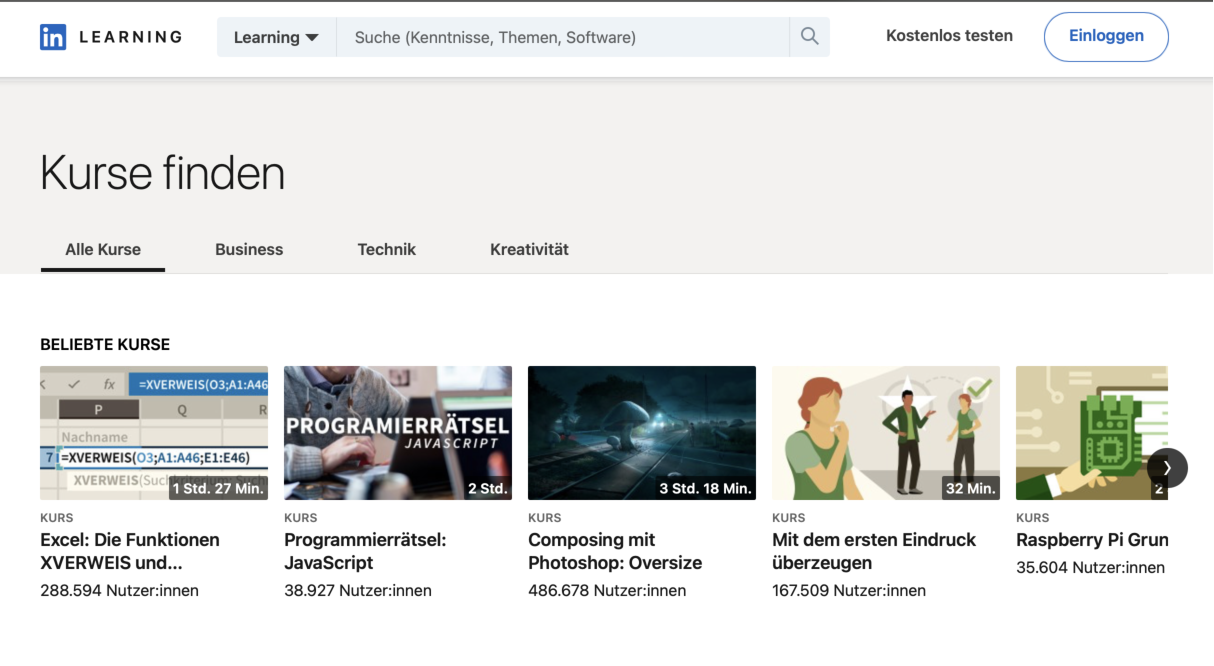
\includegraphics[width=0.3\textwidth]{images/linked_in_landing.pdf}
            
\includegraphics[width=0.3\textwidth]{images/linked_in_course.pdf}
			\caption{Linked-In Learning landing-page and course overview \cite{LinkedInLearningMit}.}
            \label{fig:trivSol}
		\end{figure}
    
        \subsection{The Setting}
    \begin{figure}[ht!]
        \centering
        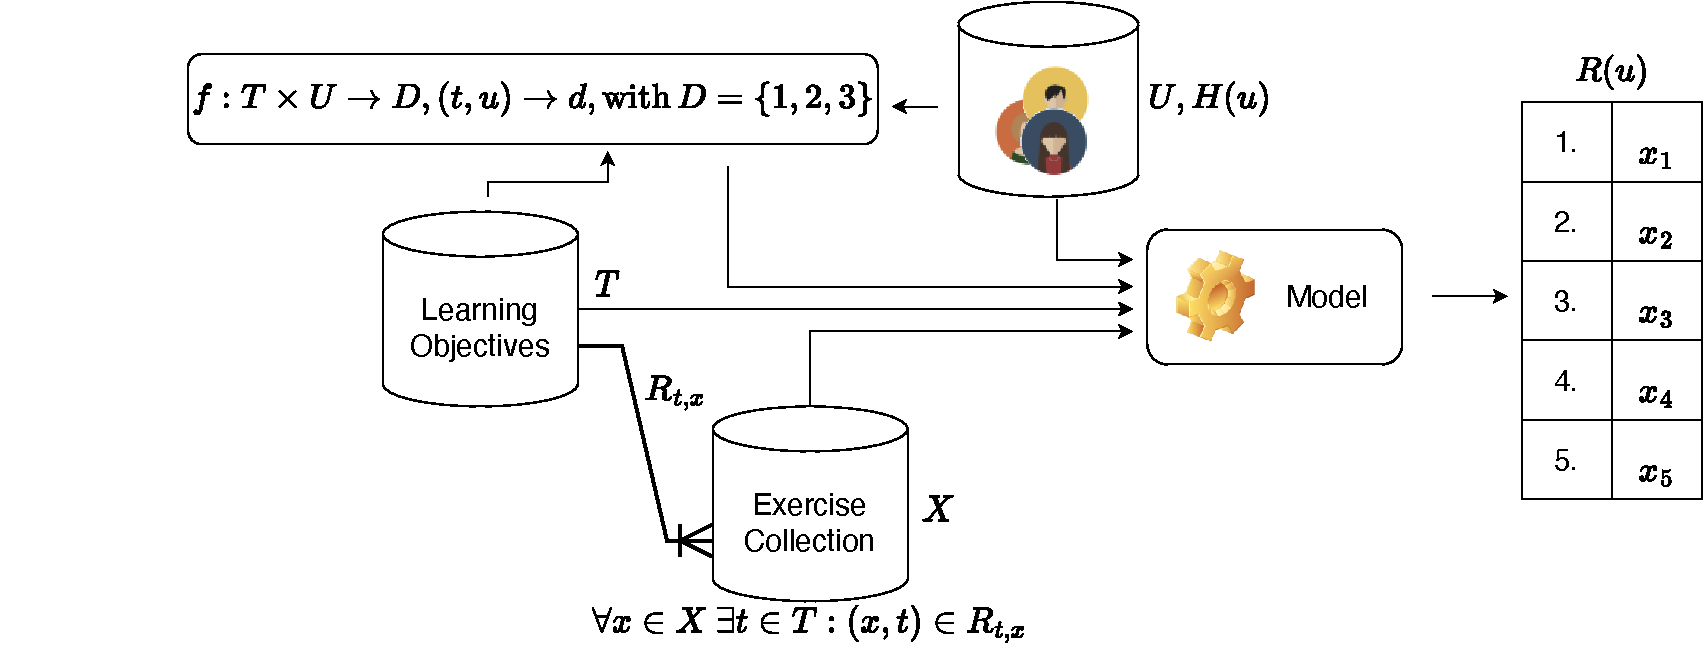
\includegraphics[width=0.6\textwidth]{images/setting.pdf}
        \caption{The Setting, consisting of a user collection $U$ and their histories $h(u)$, a collection of learning objectives $T$ and a collection of exercises $X$, which can be used to predict a ranking $R(u)$ for a given user $u$.}
        \label{fig:setting}
    \end{figure}

    \subsection{Model Adaption}
    \begin{figure}[ht!]
        \centering
        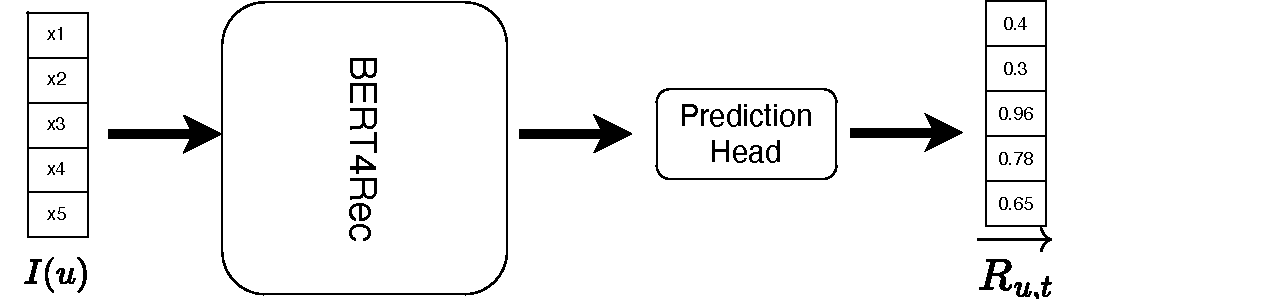
\includegraphics[width=0.4\textwidth]{images/cbf.pdf}
        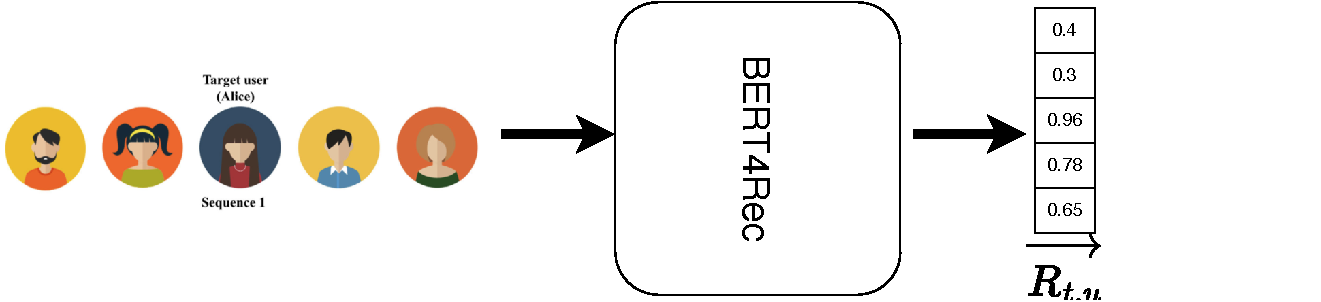
\includegraphics[width=0.4\textwidth]{images/CF_use_case.pdf}
        \caption{The adapted CBF-HybridBERT4Rec model on the left and the adapted CF-HybridBERT4Rec model on the right.}
        \label{fig:modelAdapt}
    \end{figure}

    \begin{equation}
        H(u) := (\{(x_i, t_j, s_k)| (x_i, t_j) \in R_{t,x}\}, \leq)
    \end{equation}
    \begin{equation}
        I(u) := (\{x_i|(x_i, t_j, s_k) \in H(u)\}, \leq)
    \end{equation}

    \begin{equation}
        u \in N \iff d_{u, t} = d_{u_m, t} \text{\,} \wedge (x, t) \in \{(x,t)|(x,t,s_k) \in H(u)\}
    \end{equation}

    \begin{algorithm}[ht!]
        \caption{HybridBERT4Rec in an E-Learning Setting}
        \begin{algorithmic}[1]
            \ForAll{$u_m \in U$}
                \State $r_{x,u_m} = \texttt{cbf\_hybridbert4rec}(H(u_m))$
                \ForAll{$(x,t) \in R_{t,x}$}
                    \State $r_{u, x} = \texttt{cf\_bert4rec}(u_m,t,x)$
                    \State $\hat{r}_{u,x} = \texttt{prediction\_layer}(r_{x,u}, r_{u,x})$
                \EndFor
            \EndFor
        \end{algorithmic}
    \end{algorithm}

    \FloatBarrier
    \subsection{Solving Evaluation}
    ABC
    \subsection{Remaining Possible Issues}
    ABC
    \section{Conclusion}
    ABC
%TC:ignore
%\clearpage %add new page for references
    \singlespacing
    \emergencystretch 3em
    \hfuzz 1px
    \printbibliography[heading=bibnumbered]

% \clearpage
% \begin{appendices}

% \section{Here go any appendices!}

% \end{appendices}

%TC:endignore
\end{document}